\chapter{New Features For Resources}

With the new Projectmechanism in OpenCms 4.4 come several new
features for resources in the offline project.

These features are:
\begin{itemize}
\item Undelete resources that are marked as deleted.
\item Undo changes of a resource by restoring the online information.
\item Restore versions of a file from the history.
\item Publish single files or folders directly.
\item Copy resources to an existing project.
\end{itemize}

\newpage
\section{Undelete resources}
\index{undelete}
When a resource that already exists in the online
project is deleted it is marked by crossing out its entry in the
file list. Now it is possible to undelete these resources. When
undeleting a folder all subresources in this folder that were
marked as deleted are undeleted, too. You must have write access
to undelete a resource.

\begin{figure}[hbt]
\begin{center}
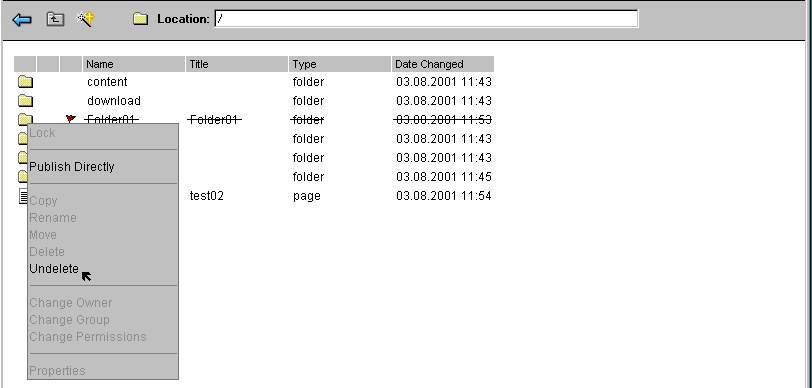
\includegraphics[width=\sgw]
                   {pics/newProject/undel03}
\caption[Undelete a resource]
           {Undelete a resource}
\label{undel}
\end{center}
\end{figure}

After the resource is undeleted its state is set to changed and
the resource is locked by the current user.

\newpage
\section{Undo changes}
\index{undo}

Changes of a resource can now be undone. The resource must be
marked as changed and it must be locked. You must have write
access to the resource. When the changes of a folder are undone
all changes of subresources are undone, too. This feature copies
the information from the online project, so all changes that were
not published are lost and new resources are deleted.

\begin{figure}[hbt]
\begin{center}
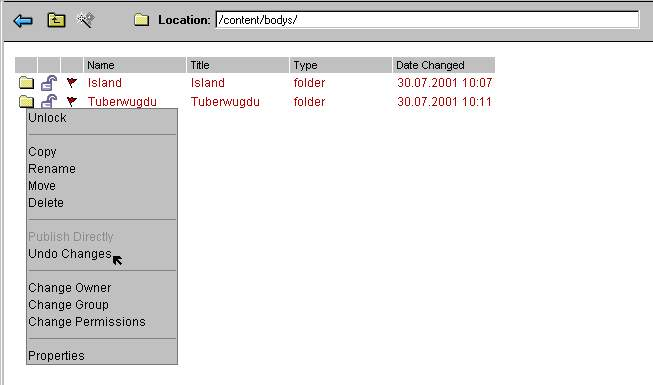
\includegraphics[width=\sgw]
                   {pics/newProject/undo01}
\caption[Undo changes of a resource]
           {Undo changes of a resource}
\label{undo}
\end{center}
\end{figure}


\newpage
\section{Restore a version from history}
\index{history}

Now older versions of a file can be restored from the history. The
file must be locked. This feature currently works only for files
not for folders. The function is only enabled for locked files. It
is implemented in the detail view of the history.

You have to choose the version from the list of versions and click
on the detail button. To restore the version click on the "Restore
version"-button. You must have write access to the file if you
want to restore a version.

\begin{figure}[hbt]
\begin{minipage}[b]{0.499\linewidth}
\begin{center}
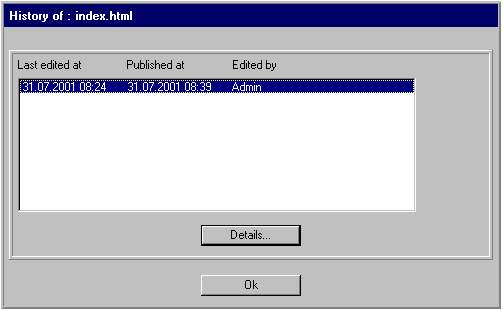
\includegraphics[width=\sgw]
                   {pics/newProject/restore01}
\end{center}
\end{minipage}
\begin{minipage}[b]{0.499\linewidth}
\begin{center}
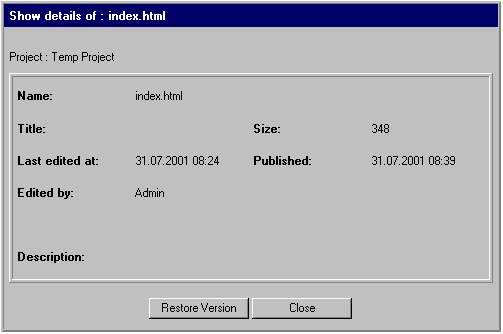
\includegraphics[width=\sgw]
                   {pics/newProject/restore02}
\end{center}
\end{minipage}
\caption[Restore a version]
           {Restore a version}
\label{restorever}
\end{figure}


\newpage
\section{Publish a resource}
\index{publish resource}

Resources can now be published directly. They must be unlocked to
enable the function in the context menu. Only the projectmanager
and the administrator are allowed to publish resources.

\begin{figure}[hbt]
\begin{center}
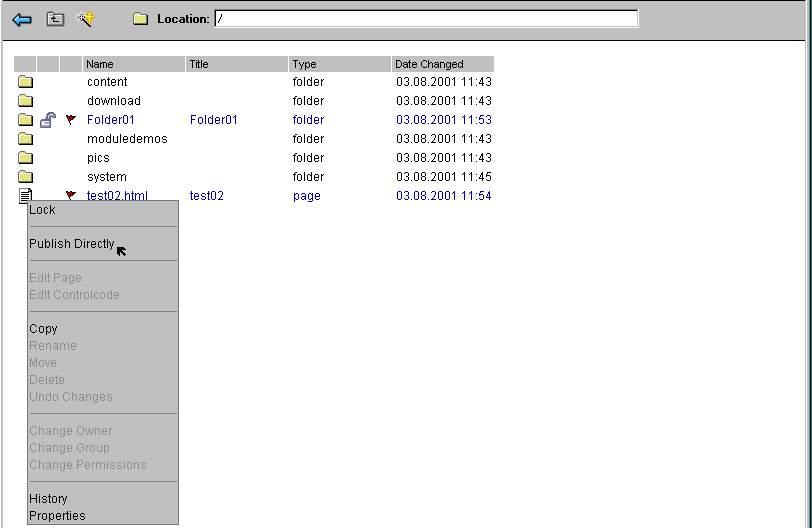
\includegraphics[width=\sgw]
                   {pics/newProject/publish03}
\caption[Publish a resource]
           {Publish a resource}
\label{publishres}
\end{center}
\end{figure}

When a resource is published directly

\begin{itemize}
\item a temporary project is created
\item the resource is copied to the new project
\item the projectid of the resource and all its subresources is set to the new project
\item the new project is published and deleted.
\end{itemize}


\newpage
\section{Copy a resource to the project}

A resource that does not belongs to the current offline project is
colored grey. You can copy this resource to the current offline
project with this new feature in the context menu. Only the
projectmanager and the administrator are allowed to copy resources
to the project.

\begin{figure}[hbt]
\begin{center}
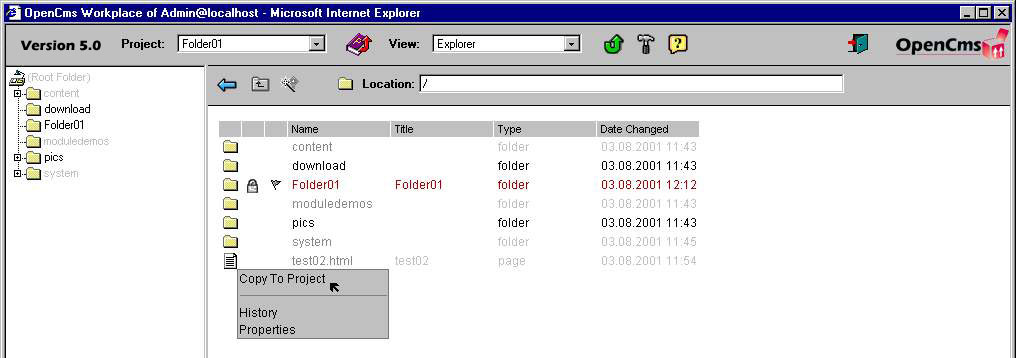
\includegraphics[width=\sgw]
                   {pics/newProject/copyPro02}
\caption[Copy a resource to project]
           {Copy a resource to project}
\label{copytoproject}
\end{center}
\end{figure}

You can also copy the parent resource of an already existing
resource to the project, but it is not possible to copy the root
folder to an existing project. For this you must create a new
project.
